\documentclass[12pt,letterpaper]{article}

\RequirePackage{xcolor}
\definecolor{tecAzul}{cmyk}{1,0.91,0.33,0.25} % según manual de imagen 2016
\definecolor{tecRojo}{cmyk}{0,0.9,0.86,0}     % según manual de imagen 2016
\definecolor{comando}{cmyk}{0,0.9,0.50,0} 
\renewcommand{\familydefault}{\sfdefault}

\usepackage[spanish,es-tabla]{babel}

\usepackage{titlesec}
\titleformat*{\section}%
{\normalfont\Large\bfseries\color{tecAzul}}
\titleformat*{\subsection}%
{\normalfont\large\bfseries\color{tecAzul}}


\usepackage[tmargin=2cm,bmargin=2cm,lmargin=2.5cm,rmargin=2.5cm]{geometry}
\usepackage{textpos}
\usepackage{tikz}
\usepackage{pgfplots}
\usepackage{pgf}
\usepackage{graphicx}
\usepackage{float}
\usepackage{array}
\usepackage{amssymb}
\usepackage{hyperref}
\usepackage{comment}
\usepackage{subfig}
\usepackage{listings}
\usepackage[margin=1cm]{caption}


%
% paragraph layout
%
\parindent0em                           % indentation width of first line
\parskip1.3ex                           % space between paragraphs


\title{Control Óptimo}

\newcommand{\EstudianteA}{Araya Fallas, Gerardo Enrique, gaf1@estudiantec.cr.}

\pgfplotsset{compat=1.17}

\begin{document}
	
\graphicspath{{./}{./fig/}}

%-------------------------- Title section -------------------------------------%

% kit logo
\begin{textblock}{10}[0,0](-0.5,0)
	\begin{flushleft}
		\large 
		Escuela de Ingeniería Electrónica \\
		Licenciatura en Ingeniería Electrónica \\
		EL4419 Análisis y Control de Sistemas Lineales\\
		I Semestre 2023
	\end{flushleft}
\end{textblock}

%Institute and Chair
\begin{textblock}{10}[0,0](2.9,-0.35)
	\begin{flushright}
		
\includegraphics[scale=0.8]{Firma_TEC-4.pdf}
	\end{flushright}
\end{textblock}

%% Title %%
\begin{center}
	\vspace{2.0cm}
	%{\Large\color{tecRojo} Tutorial de Proyecto }
	\par\vspace{.3cm}
	{\LARGE\bf\color{tecAzul}{Control Optimo}}
	\par\vspace{.3cm}
	{\large{\EstudianteA} 
	\vspace{0.3cm}}
\end{center}


%------------------------------------------------------------------------------%


%\begin{abstract}
%Resumen sobre el contenido del reporte y el trabajo realizado como parte del 
%proyecto.
%\end{abstract}

\section{Introducción}
El Control Óptimo es producto del desarrollo de la Teoría de Control la cual tiene sus inicios a partir del año 1868, por medio de los postulados de J.C. Maxwell  que se baso en el modelo de ecuación
diferencial del regulador de Watt y analizando su estabilidad \cite{Teoría}
Para 1960 se generan las tres primeras publicaciones referentes al Control Óptimo generado por R.Kalman y otros co-autores, donde se desarrollo el Control de Sistemas No lineales, en el dominio temporal, el control óptimo de sistemas, suministrando
las ecuaciones de diseño para el regulador cuadrático
lineal(LQR) y l filtrado óptimo y la teoría
de estimación, suministrando las ecuaciones de diseño para
el filtro digital.\cite{Teoría}
Se puede decir que un  Control es Optimo,. si es capaz de minimizar el costo (en términos de implementación) de diversos requerimientos y especificaciones \cite{Catedra}
%------------------------------------------------------------------------------%

\section{Marco Teórico}

\subsubsection{El principio del Máximo de Pontryagin}

Dicho principio se basa en el postulado realizado por el Ruso Lev Semyonovich Pontryagin, matemático, ciego desde sus catorce años. Dicho postulado hace referencia al siguiente procedimiento:
\cite{Mariano} 
\begin{figure}[H]
    \centering
    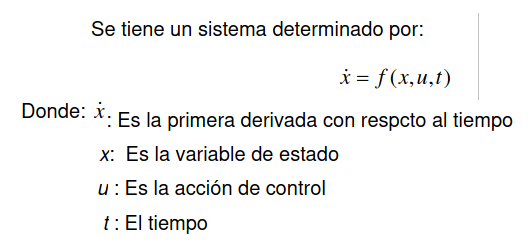
\includegraphics[scale=0.55]{EL5841_reporte/im05.png}
    \caption{Principio Máximo \cite{Mariano} } 
    \label{fig:MV4}
\end{figure}
Se desea optimizar, es decir determinar el máximo y mínimo de la función, que corresponde al indice de comportamiento 
\begin{figure}[H]
    \centering
    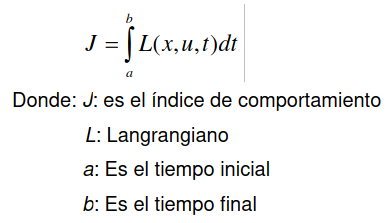
\includegraphics[scale=0.55]{EL5841_reporte/im07.png}
    \caption{Índice de Comportamiento \cite{Mariano}   }
    \label{fig:MV4}
\end{figure}
El problema consiste en hallar el control óptimo u = f(x(t),t) que minimice el índice de comportamiento J sobre el intervalo [a,b].\cite{Mariano} Para su solución el Principio de Pontryagin usa el método de los multiplicadores de Lagrange de la siguiente forma:

Primer Paso: se forma la función de Pontryagin H dada por:
\begin{figure}[H]
    \centering
    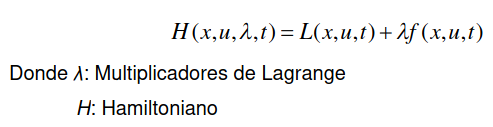
\includegraphics[scale=0.55]{EL5841_reporte/im08.png}
    \caption{función de Pontryagin H \cite{Mariano}   }
    \label{fig:MV4}
\end{figure}
Segundo Paso: se resuelve la ecuación:
\begin{figure}[H]
    \centering
    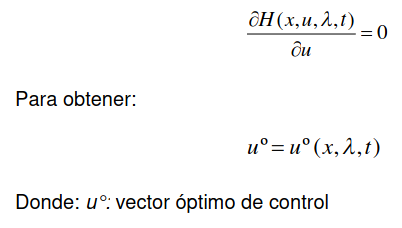
\includegraphics[scale=0.55]{EL5841_reporte/im09.png}
    \caption{Vector óptimo de control H \cite{Mariano}   }
    \label{fig:MV4}
\end{figure}
Tercer Paso: Encontrar la función H optimizada
\begin{figure}[H]
    \centering
    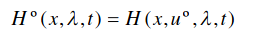
\includegraphics[scale=0.55]{EL5841_reporte/im10.png}
    \caption{Función H optimizada \cite{Mariano}   }
    \label{fig:MV4}
\end{figure}
Cuarto Paso: Encontrar las ecuaciones canonicas diferenciales
\begin{figure}[H]
    \centering
    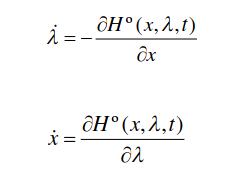
\includegraphics[scale=0.55]{EL5841_reporte/im11.png}
    \caption{Ecuaciones canonicas diferenciales \cite{Mariano}   }
    \label{fig:MV4}
\end{figure}

para poder determinar que tan bueno es la optimización existe un indice de Performace \cite{Mariano}.

\begin{figure}[H]
    \centering
    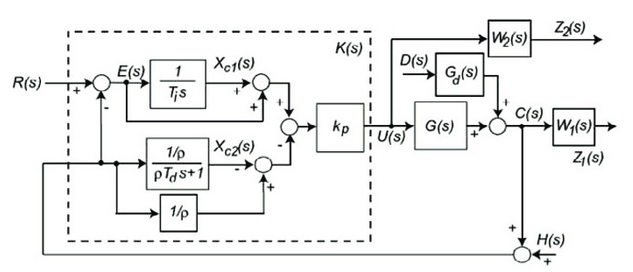
\includegraphics[scale=0.55]{EL5841_reporte/im12.png}
    \caption{Diagrama de bloques. Optimización del control \cite{Goncalves}}   \label{fig:MV4}
\end{figure}

\begin{figure}[H]
    \centering
    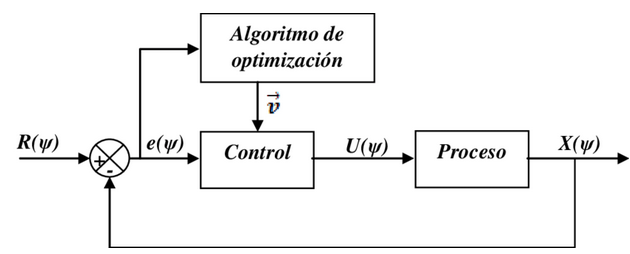
\includegraphics[scale=0.55]{EL5841_reporte/im13.png}
    \caption{Diagrama de bloques. Algoritmo de optimización \cite{Goncalves}}   \label{fig:MV4}
\end{figure}

\\
\
\

%------------------------------------------------------------------------------%







%------------------------------------------------------------------------------%
\begin{thebibliography}{1}

\bibitem{Teoría}
TEORÍA DE CONTROL INTRODUCCIÓN. (n.d.). http://www3.fi.mdp.edu.ar/control4c7/APUNTES /Clase%201%20-%20Introduccion%20-%20Modelado.pdf

\bibitem{Mariano}
Mariano, L., Malagón, S.
Andrés, O., León, A.(2009).
Introducción al Control Óptimo y aplicación del Principio de Pontryagin al comportamiento de un motor de Corriente Continua. 
https://repository.upb.edu.co/bitstream/handle/20.500.11912/599/digital18243.pdf?sequence.
‌
\bibitem{Mantz}
‌Mantz, R. (2003). 
Introducción al controlóptimo.https://catedra.ing.unlp.edu.ar/electrotecnia/control/electronica/archivos/apuntesc.optimo.pdf.

\bibitem{Goncalves}
‌https://www.researchgate.net/figure/Figura-6-Diagrama-de-bloques-
para-la-optimizacion-del-controlador-PID-Goncalves
-etl

\bibitem{Guillen}
Guillen, A., Cerrada, C., Cerrolaza, M.,  Grande -Caracas -Venezuela, S. (1989).
AJUSTE OPTIMO DE FUNCIONES DE TRANSFERENCIA UTILIZADAS PARA LA IDENTIFICACION DE PARAMETROS DE ROBOTS INDUSTRIALES. 
Revista Internacional de Métodos Numéricos Para Cáiculo Y Diseño En Ingeniería,5, 359–378.
https://upcommons.upc.edu/bitstream/handle/2099/8776/Article04.pdf?sequence


\bibitem{Tremante}
P. Tremante y E. Brea, “Ingeniería Industrial. Actualidad y Nuevas Tendencias”, Redalyc.org. [En línea]. Disponible en: https://www.redalyc.org/pdf/2150/215037911010.pdf. [Consultado: 23-oct-2023].





\end{thebibliography}
\end{document}









